\documentclass[11pt,a4paper]{article}
\usepackage[spanish,es-nodecimaldot]{babel}	% Utilizar español
\usepackage[utf8]{inputenc}					% Caracteres UTF-8
\usepackage{graphicx}						% Imagenes
\usepackage[hidelinks]{hyperref}			% Poner enlaces sin marcarlos en rojo
\usepackage{fancyhdr}						% Modificar encabezados y pies de pagina
\usepackage{float}							% Insertar figuras
\usepackage[textwidth=390pt]{geometry}		% Anchura de la pagina
\usepackage[nottoc]{tocbibind}				% Referencias (no incluir num pagina indice en Indice)
\usepackage{enumitem}						% Permitir enumerate con distintos simbolos
\usepackage[T1]{fontenc}					% Usar textsc en sections
\usepackage{amsmath}						% Símbolos matemáticos
\usepackage[simplified]{pgf-umlcd}
\usepackage{pdflscape}
\usetikzlibrary{babel} % Problemas del español al usar <,> para las citas
\usepackage{typearea} % Paginas horizontales

\usepackage{listings}
\usepackage{xcolor}
 
\definecolor{codegreen}{rgb}{0,0.6,0}
\definecolor{codegray}{rgb}{0.5,0.5,0.5}
\definecolor{codepurple}{rgb}{0.58,0,0.82}
\definecolor{backcolour}{rgb}{0.95,0.95,0.92}
 
\lstdefinestyle{mystyle}{
    backgroundcolor=\color{backcolour},   
    commentstyle=\color{codegreen},
    keywordstyle=\color{magenta},
    numberstyle=\tiny\color{codegray},
    stringstyle=\color{codepurple},
    basicstyle=\ttfamily\footnotesize,
    breakatwhitespace=false,         
    breaklines=true,                 
    captionpos=b,                    
    keepspaces=true,                 
    numbers=left,                    
    numbersep=5pt,                  
    showspaces=false,                
    showstringspaces=false,
    showtabs=false,                  
    tabsize=4,
    language=Python
}
 
\lstset{style=mystyle}

% Comando para poner el nombre de la asignatura
\newcommand{\asignatura}{Nuevos Paradigmas de Interacción}
\newcommand{\autorv}{Vladislav Nikolov Vasilev}
\newcommand{\autorj}{José María Sánchez Guerrero}
\newcommand{\autorf}{Fernando Vallecillos Ruiz}
\newcommand{\titulo}{Práctica Gestos}
\newcommand{\subtitulo}{Memoria Técnica}


% Configuracion de encabezados y pies de pagina
\pagestyle{fancy}
\lhead{Vladislav, José María, Fernando}
\rhead{\asignatura{}}
\lfoot{Grado en Ingeniería Informática}
\cfoot{}
\rfoot{\thepage}
\renewcommand{\headrulewidth}{0.4pt}		% Linea cabeza de pagina
\renewcommand{\footrulewidth}{0.4pt}		% Linea pie de pagina


% new pagestyle
\fancypagestyle{lscape}{
  \headwidth\textwidth
}

\begin{document}
\pagenumbering{gobble}

% Pagina de titulo
\begin{titlepage}

\begin{minipage}{\textwidth}

\centering

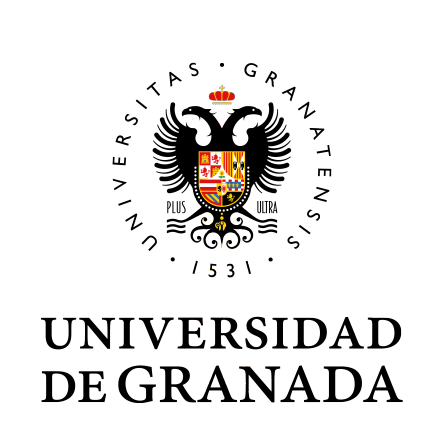
\includegraphics[scale=0.5]{img/ugr.png}\\

\textsc{\Large \asignatura{}\\[0.2cm]}
\textsc{GRADO EN INGENIERÍA INFORMÁTICA}\\[1cm]

\noindent\rule[-1ex]{\textwidth}{1pt}\\[1.5ex]
\textsc{{\Huge \titulo\\[0.5ex]}}
\textsc{{\Large \subtitulo\\}}
\noindent\rule[-1ex]{\textwidth}{2pt}\\[3.5ex]

\end{minipage}

\vspace{0.5cm}

\begin{minipage}{\textwidth}

\centering

\textbf{Autores}\\ {\autorv{}}\\{\autorj{}}\\{\autorf{}}\\[2.5ex]
\textbf{Rama}\\ {Computación y Sistemas Inteligentes}\\[2.5ex]
\vspace{0.3cm}


\includegraphics[scale=0.3]{img/etsiit.jpeg}

\vspace{0.5cm}
\textsc{Escuela Técnica Superior de Ingenierías Informática y de Telecomunicación}\\
\vspace{0.5cm}
\textsc{Curso 2019-2020}
\end{minipage}
\end{titlepage}

\pagenumbering{arabic}
\tableofcontents
\thispagestyle{empty}				% No usar estilo en la pagina de indice

\newpage

\setlength{\parskip}{1em}


\section{Introducción}
En este proyecto vamos a explicar nuestra \textit{Natural User Interface (NUI)} que hará que nuestra visita a la Alhambra sea más
dinámica y productiva. El proyecto constaría de varios dispositivos, como pueden ser principalmente unas gafas de realidad aumentada,
un dispositivo \textit{Leap Motion} y un micrófono integrados en las gafas, y un \textit{smartphone} que utilizaremos tanto para
manejar el sistema gracias a los múltiples sensores que incorpora como para controlar la aplicación.

En esta segunda versión del proyecto vamos a encargarnos de la interfaz por gestos, es decir, dejaremos a un lado los sensores
y el controlador por voz. Vamos a encargarnos de la realidad aumentada y los gestos para manejar el sistema.

\section{Interfaz por gestos}
Como no disponemos de unas gafas con un Leap Motion incorporado, vamos a realizar nuestra simulación en un programa de \texttt{Python} aparte. En
nuestra versión, la opción de utilizarlo verticalmente no está disponible, por lo que su funcionamiento se mostrará con el dispositivo
sobre la mesa. Se han implementedo los siguientes gestos: \textit{click}, \textit{swipe}, zoom y agarre y movimiento. Un
poco más adelante vamos a describir en qué consiste cada gesto y diremos muy brevemente cómo se ha
implementado cada uno de ellos.

\section{Información y estructuras de datos utilizadas}

En esta sección se describirán las especificaciones de nuestra clase principal. Así como diferentes estructuras utilizadas en nuestro código para hacer posible una pequeña interfaz gráfica. Esta permitirá al usuario ver de una forma visual los resultados de nuestro proyecto.

\subsection{Clase Leap}

Nuestra clase \texttt{LeapMotionListener}, se trata de nuestra única clase con los métodos necesarios para poder controlar la información recibida a través del dispositivo.

Esta clase consta de cinco métodos los cuales se explican por sí mismos. Sin embargo, se podrían destacar dos métodos:

\begin{itemize}[label=\textbullet]
	\item \texttt{on\_connect}: este método es llamado cuando el dispositivo ha sido conectado.
	La relevancia de este método se encuentra en que permite el reconocimiento de los diferentes gestos implementados en la clase. A pesar de que solo utilizaremos uno de estos gestos en nuestro proyecto, hemos encontrado que el habilitarlos todos produce una reducción de la malinterpretación de estos.
	\item \texttt{on\_frame}: Este método será llamado por cada frame que recibamos desde el dispositivo.
	Se podría considerar como nuestro método principal. Ya que el número de frames por segundo fluctúa dependiendo de la capacidad de la máquina, decidimos, por el bien de la eficiencia, intentar reducir en número de llamadas a funciones al mínimo.
\end{itemize}


Además hemos hecho uso del objeto \texttt{InteractionBox}. Este objeto representa una región en forma caja en el campo de vista del \texttt{LeapMotion}. Esta región es usada para mapear la posición de las manos en el área. Si bien parece una opción fácil de usar, existe el problema del tamaño de esta región. Se puede apreciar en la siguiente imágen:

\begin{figure}[H]
\centering
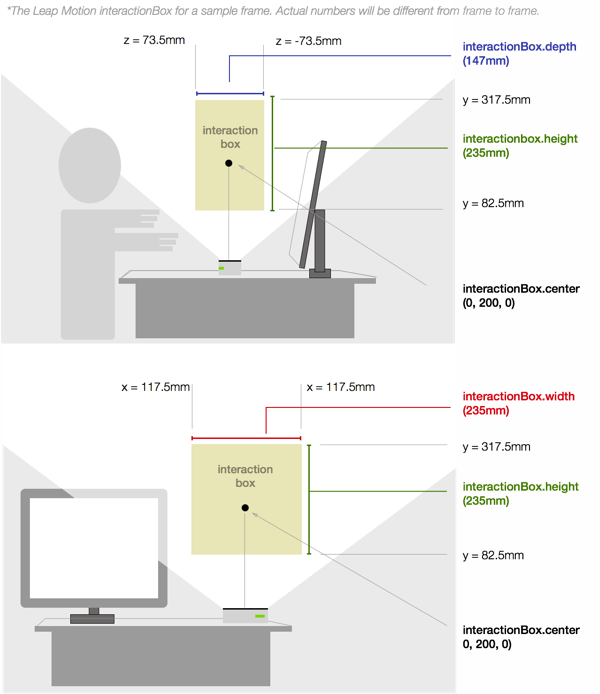
\includegraphics[scale=0.5]{img/box.png}
\end{figure}

Como se puede apreciar, la región es apenas $15 \times 20 \times 20$ aunque la visión del dispositivo sea bastante mayor. 
Existe una solución simple para “aumentar” la región de interacción. Esta solución hace uso de la capacidad de modificar las coordenadas antes de normalizarlas con respecto a la caja. Si dividimos las coordenadas previas a la normalización entre dos, resulta en un efecto de ``despliegue'' de la caja original, al doble de su tamaño. 
Hemos realizado esta modificación al Eje-x y Eje-z. A pesar de que contradecimos el objetivo del ``mapeo perfecto'' de la clase \texttt{Interaction Box}, esta solución ha sido propuesta por desarrolladores profesionales de \textit{LeapMotion}.

\subsection{Interfaz Gráfica}

A diferencia de nuevas versiones de \textit{LeapMotion}, los kit de desarrollo en \texttt{Python} no tienen una interfaz gráfica. Esto nos dejaba dos opciones posibles:

\begin{itemize}[label=\textbullet]
	\item Mostrar resultados por la terminal a través del método\texttt{on\_frame}.
	\item Crear nuestra propia interfaz gráfica para mostrar los resultados.
\end{itemize}

Nos decidimos por la segunda opción y gracias a la biblioteca \texttt{tkinter}, desarrollamos una forma de visualización de nuestro proyecto.
De una forma simplificada, \texttt{tkinter} es una biblioteca que permite creación de ventanas donde mostrar texto y/o imágenes. Haciendo uso de variables globales y funciones recursivas en intervalos, hemos conseguido una forma simple y eficiente de representar cambios a tiempo real.
Como ha sido mencionado antes, la necesidad por un método lo más óptimo posible que interfiriera lo mínimo con la velocidad de procesamiento de frames del dispositivo era prioridad. 

Para este objetivo hacemos uso de:

\begin{itemize}[label=\textbullet]
	\item Variables globales: la declaración de variables globales, en contraste con variables locales o copia de variables en métodos, permite incrementar la agilidad del programa al acceder a ellas.
	\item Métodos de actualización de la ventana independiente de la frecuencia del dispositivo: los límites de las máquinas se hacían muy presentes en este punto. La frecuencia del dispositivo es muy alta (y variable) y la capacidad de actualización de la ventana en comparación, era demasiado lenta. Si tuviésemos los recursos suficientes, sería posible un actualización completamente a tiempo real solo dependiendo de los frames, sin embargo nuestra versión crea una ilusión bastante cerca al tiempo real (cada 50 ms).
\end{itemize}

\section{Descripción de los gestos}

En esta sección se van a describir todos los gestos que se han implementado. Se va
a hacer una breve descripción de en qué consiste y se va a mostrar muy por encima
el código asociado en los casos en los que se haya considerado necesario (cuando
lo que se quiere mostrar es relevante ya que se trata de algo no trivial).

Antes de continuar, hay que destacar que algunos de los gestos solo están disponibles
cuando ambas manos están encima del \textit{Leap Motion}. Por ejemplo, el \textit{click},
el \textit{swipe} y el agarre y movimiento solo pueden ser realizados cuando se detecta
una única mano. El zoom solo se puede realizar si se han detectado dos manos y se hace
el gesto correspondiente con los dedos. Para comprobar si se usa una mano o dos, podemos
hacer los siguiente:

\begin{lstlisting}
if(len(frame.hands) == 1):
	...

f(len(frame.hands) >= 2 ):
	...
\end{lstlisting}

En este caso, comprobamos si se han detectado dos o más manos, ya que puede pasar que
otra persona pase la mano por encima del dispositivo. Sin embargo, nos quedamos siempre
con las dos primeras manos que hayamos detectado.

\subsection{Descripción del \textit{click}}

Este gesto sirve para mostrar información extra sobre el objeto. El gesto consiste en cerrar y abrir el puño en la zona sobre la que
queremos obtener información. Esta zona se detectaría automáticamente mediante un algoritmo implementado en las gafas, pero como no disponemos
de dicha tecnología, utilizaremos una imagen fija con una zona resaltada

Esto mostrará en la interfaz de nuestras gafas de realidad aumentada una imagen de la zona resaltada, junto con información de esta. La
información podrá ser modificada mediante otros gestos descritos posteriormente.

Para saber si estamos haciendo o no un \textit{click}, simplemente tenemos que
comprobar la siguiente condición:

\begin{lstlisting}
if (closed_hand and hands[0].grab_strength == 1.0):
	...
\end{lstlisting}

Después se va a comprobar si la mano está posicionada en la zona adecuada, en cuyo caso se
mostrará la imagen que contiene información.

\subsection{Descripción del \textit{swipe}}

Al igual que mostramos la información con el gesto anterior, necesitaremos otro gesto para ocultarla. Nosotros utilizamos el \textit{swipe}, el cual
detectará los movimientos en el eje X. De esta formá, podrá ser usado tanto por personas zurdas como diestras sin ningún tipo de problema.
Modificaremos el parámetro de su velocidad para que no se pueda confundir con otros gestos que hacemos naturalmente.

La implementación es la siguiente:

\begin{lstlisting}
if (len(frame.gestures()) != 0):
	# Check if the hand is completely open and the gesture is swiping
	if open_hand and (frame.gestures()[0].type == Leap.Gesture.TYPE_SWIPE):
		swipe = SwipeGesture(frame.gestures()[0])
		# Check that the main direction of the swipe is the x-axis (left or right)
		if(abs (swipe.direction[0]) > 0.7):
			swiping = True
\end{lstlisting}

Simplemente estamos comprobando si se ha detectado algún gesto y si ese gesto
se ha realizado con la mano abierta y es un \textit{swipe} en cualquier sentido
en el eje X.

Como se puede ver, estamos utilizando un gesto que ya viene en \textit{Leap}, aunque
lo estamos adaptando a nuestras necesidades, ya que hemos limitado su funcionamiento
al eje X.

\subsection{Descripción del zoom}

Este gesto sirve para disminuir o aumentar el tamaño de la información mostrada. Para utilizar este gesto tendremos que tener las dos manos
sobre la zona de detección del \textit{Leap Motion} y, posteriormente, extender los dedos pulgar e índice con una apertura mínima entre ellos de 40º.
El zoom que se le aplicará a la imagen será directamente proporcional a la distancia en el eje X entre la mano derecha y la mano izquierda. La
implementación de dicho gesto es la siguiente:

\begin{lstlisting}
# Let's check if both hands have only the thumb and index extended
two_up_left = True
two_up_right = True

for i in range(0, 2):
	two_up_left = two_up_left and left_hand.fingers[i].is_extended
    two_up_right = two_up_right and right_hand.fingers[i].is_extended

for i in range(2, 5):
	two_up_left = two_up_left and not left_hand.fingers[i].is_extended
    two_up_right = two_up_right and not right_hand.fingers[i].is_extended

# Set the minimum angle between thumb and index to be considered zooming
threshold_angle = 40

# If they have the left index and thumb extended, we calculate the angle
if two_up_left:
	vec1 = left_hand.fingers[0].direction    # Thumb
	vec2 = left_hand.fingers[1].direction    # Index
    angle1 = acos(max(-1.0, min(1.0, vec1.dot(vec2)))) * Leap.RAD_TO_DEG

    # Check if the angle is open enough
    if (angle1 > threshold_angle):
    		left_hand_zoom = True
	else:
    		left_hand_zoom = False
else:
	left_hand_zoom = False

# If they have the right index and thumb extended, we calculate the angle
if two_up_right:
	vec1 = right_hand.fingers[0].direction    # Thumb
    vec2 = right_hand.fingers[1].direction    # Index
    angle2 = acos(max(-1.0, min(1.0, vec1.dot(vec2)))) * Leap.RAD_TO_DEG

    # Check if the angle is open enough
    if (angle2 > threshold_angle):
    		right_hand_zoom = True
	else:
		right_hand_zoom = False
else:
	right_hand_zoom = False
\end{lstlisting}

Básicamente, lo que se hace es comprobar si los dedos índice y pulgar de las dos
manos están extendidos y el resto cerrados. Después, se comprueba si en cada
caso el ángulo que forman es mayor que 40º, en caso de que la condición anterior
se haya satisfecho.

Además de hacer zoom, también está implementada una función que, si llegamos a un umbral de zoom en algunas zonas determinadas (por ejemplo,
a la fuente de la funete de los leones, o una habitación del Palacio de Carlos V), mostraremos información más detallada sobre ésta. La
implementación es la siguiente?? o ya la hemos puesto antes???


\subsection{Descripción del agarre y movimiento}

Para mover la información sobre toda la superficie de las gafas de realidad aumentada, utilizaremos el siguiente gesto. Cerraremos el puño
(tendrá que ser en las mismas coordenadas sobre las que está la información, para así evitar moverla sin querer con algún gesto natural) y
posteriormente la moveremos al lugar que queramos. Para dejar de moverla, simplemente volvemos a abrir la mano.

Si estamos arrastrando la información fuera de nuestro campo de visión, hemos puesto unos límites tanto vertical como horizontalmente, para que
el programa no nos permita hacerlo.

Arrastrada la información, también guardaremos las propiedades que conservaba previamente, como por ejemplo, si le habíamos hecho zoom, o la
habíamos arrastrado en otro momento.

Para comprobar que estamos haciendo un agarre con la mano, tenemos que
comprobar la misma condición que con el \textit{click}, aunque lo que se va
a ejecutar va a ser diferente, ya que se va a actualizar la posición de la
imagen en función del movimiento realizado, respetando siempre los bordes
que se hayan impuesto.

\newpage

\begin{thebibliography}{5}
\end{thebibliography}

\end{document}

